\section{落下間隔変化における高速化への影響}
先行研究\cite{ref:8-5}にて,等間隔の時間で物体を落下させると,落下速度が一定になることが報告されている.これは,落下によって破壊された分子構造が回復するためだと考えられる.球の落下間隔を変化させると,PAA溶液の粘性弾性回復に対して影響を与えると考えられる.これらの落下速度,高速化への影響を調査するため,落下間隔を変化させた実験を行った.

落下間隔を5分,10分,20分と変化し,球を落下させた解析した結果をFig.\ref{fig:falling-interval}に示す.縦軸は落下速度,横軸は落下開始時からの経過時間である.それぞれの場合において,超音波照射による落下球の高速化は見られた.落下間隔と落下球の終端速度の関係をFig\ref{fig:falling-interval-diff}(a)に示す.縦軸は落下球の終端速度,横軸は落下間隔である.落下間隔を変化させた場合,落下間隔が5分と10分の場合に終端速度に大きな変化は生じなかった.一方で,落下間隔が20分の場合は終端速度の分散が小さくなった.これは,弾性回復が十分に行われたため,落下中の落下速度が一定に近くなったためだと考えられる.落下間隔と高速化度合の関係をFig\ref{fig:falling-interval-diff}(b)に示す.縦軸は高速化度合,横軸は落下間隔である.落下間隔を変化させた場合,超音波照射による高速化度合に対して大きな変化が見られなかった.また,粘度比と音響境界層を球の半径で規格化した値と高速化度合の関係をFig.\ref{fig:falling-interval-diff}(c)に示す.縦軸は高速化度合,横軸は粘度比と音響境界層を球の半径で規格化した値である.粘度比と音響境界層を球の半径で規格化した値は落下間隔を変化させた場合,あまり大きく変化しなかった.これは流体物性がほぼ同一であるためと考えられる.これらの結果より,今回の実験範囲ではあまり大きな変化が現れなかったことが分かった.
\begin{figure}[H]
    \centering
    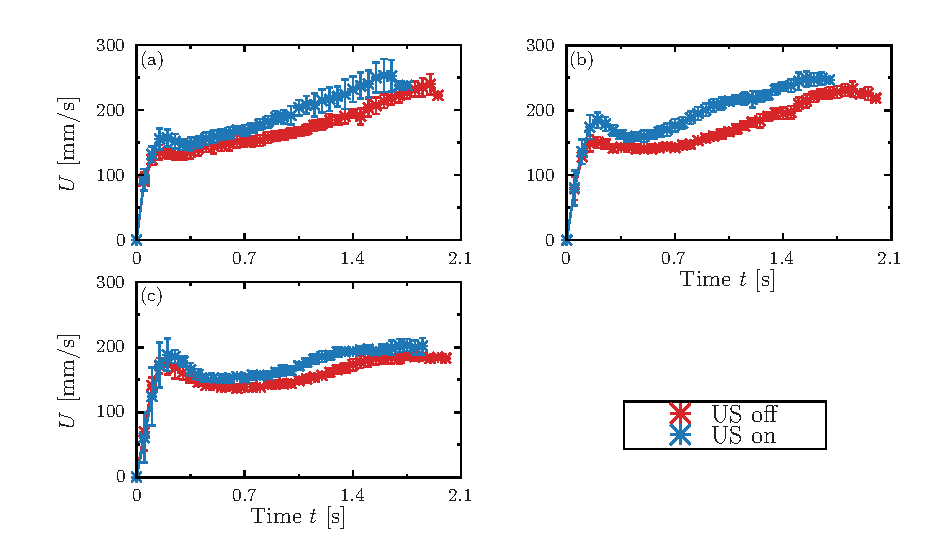
\includegraphics[width=1\textwidth]{./X-Appendix/interval/interval.eps}
    \caption{Falling speed of a sphere in 1.0wt.\%PAA solution with and without ultrasound irradiation for the interval (a)5min, (b)10min, (c)20min.}
    \label{fig:falling-interval}
\end{figure}

\begin{figure}[H]
    \centering
    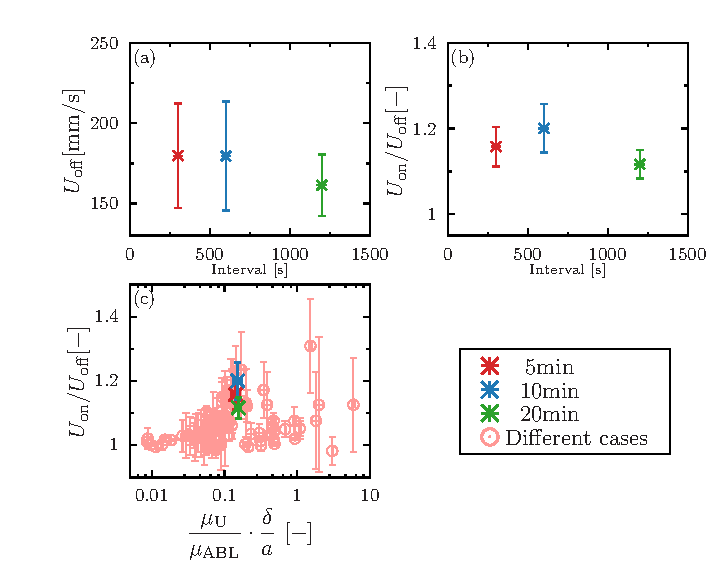
\includegraphics[width=1\textwidth]{./X-Appendix/interval/interval_cal.eps}
    \caption{ Relationship between (a)terminal velocity and interval, velocity ratio and (b) interval, (c)viscosity ratio.}
    \label{fig:falling-interval-diff}
\end{figure}
